\documentclass[11pt, onecolumn]{article}
\usepackage{geometry}
\usepackage{graphicx}
\usepackage{amssymb}
\usepackage{microtype}
\usepackage{enumitem}
\usepackage{amsmath}
\usepackage{index}
\usepackage{enumitem}
\usepackage{indentfirst}
\usepackage{setspace}
\usepackage[format=plain, font=it]{caption}
\usepackage{makecell}
\usepackage{todonotes}
\usepackage[hidelinks]{hyperref}
\usepackage{capt-of}
\geometry{a4paper, margin=2.5cm}
\singlespacing
\title{ES3J1 Group 3 Report}
\author{Anya Akram, Edward Stanley, Favour Rabiu, Matt Brooks, Nojus Plungė}
\date{\today}

\begin{document}
\setlength{\abovecaptionskip}{5pt plus 3pt minus 2pt}
\setlist{topsep=0.5em, itemsep=0em}
\setlength{\parindent}{0.5em}
\setlength{\belowcaptionskip}{-8pt}
\setlength{\belowdisplayskip}{8pt}
\pagenumbering{arabic}
\maketitle

\section*{Question 1}
\par The output produced by the motor is not smooth, so to obtain its model that can be analysed using control system theory, a filter needs to be designed.
\par The filter (and thus, the model) tuning was done according to the brief. The process followed the steps outlined below:
\begin{enumerate}
    \item The filter coefficient was set to the simplest low-pass transfer function $\frac{1}{0.1s+1}$ to start smoothing the motor output, obtained by applying the step input. An example filter performance is shown in \textit{Figure \ref{fig:q1-filter}}.
          \begin{figure}[h!]
              \centering
              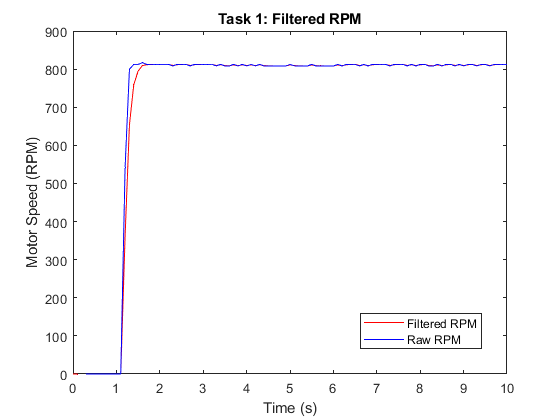
\includegraphics[width=0.6\textwidth]{q1-filter.png}
              \caption{Low-pass filter's impact on the signal.}
              \label{fig:q1-filter}
          \end{figure}
    \item The motor circuit, as set up in the brief, was assembled; the motor and Arduino were connected to the circuit and a link was established to the Simulink workspace.
    \item The motor was run using the MATLAB hardware add-on. The signal could be traced as going from the workspace input, through the PWM converter block and into the Arduino. The PWM signal generated by the Arduino then propagated through the circuit to power the motor, which had its encoder linked to the Arduino – this signal was then converted into motor revolutions per minute (RPM) in the workspace and the obtained results were designated as the output. The input into the system and the output of the motor (in RPM) was saved to the workspace for further analysis.
    \item System Identification Toolbox (SIT) was used, with the input being the signal prior being processed by the PWM block and the output being the motor's RPM.
    \item In SIT the analysis was set for the transfer function to have no zeroes and one pole – this was identified by inspection, using the unfiltered transfer function output, as the step input produced a first order response.
    \item The obtained transfer function was scaled by dividing both the numerator and the denominator by the step time ($T_s = 0.1$).
    \item The obtained transfer function was plotted against the unfiltered motor output to verify the model accuracy. If proven significantly inaccurate, the design process was repeated until a fitting filter that produced a smooth transfer function was obtained.
\end{enumerate}
\par The resulting transfer function's step response is shown in \textit{Figure \ref{fig:q1-graph}} (titled as "Computed (SIT)").
\par An alternative method for tuning the transfer function was also explored, as the steady state value of the produced function did not exactly match the motor output on the graph. The new tuning approach was found in \cite{umichControlTutorials} and was executed in the following steps:
\begin{enumerate}
    \item Steps 1-3 were repeated from the previous method: a simple low-pass filter was set up, the motor circuit was assembled and the motor response to a step input was saved to the workspace.
    \item Find the maximum gain reached by the output. This is regarded as the absolute – or steady state – gain. The value recorded was 834.
    \item The time constant for the response was calculated. This was defined as the time to reach 63.2\% of the steady-state value. In this case, a value of 528.76 RPM needed to be reached. The time to reach this value was calculated to be 1.185s. As the step was applied at $t=1$ s, the time constant was therefore $\tau = 1.185 - 1 = 0.185$s.
    \item Using the standard first order transfer function model:
          \begin{align*}
              G(s)=\frac{Y(s)}{X(s)}=\frac{K}{\tau s + 1}
          \end{align*}
          and substituting the values calculated, a final transfer function was obtained:
          \begin{align*}
              G(s)=\frac{834}{0.185s + 1}
          \end{align*}
\end{enumerate}
\par The resulting transfer function's step response is shown in \textit{Figure \ref{fig:q1-graph}} (titled as "Graphical").
\begin{figure}[h!]
    \centering
    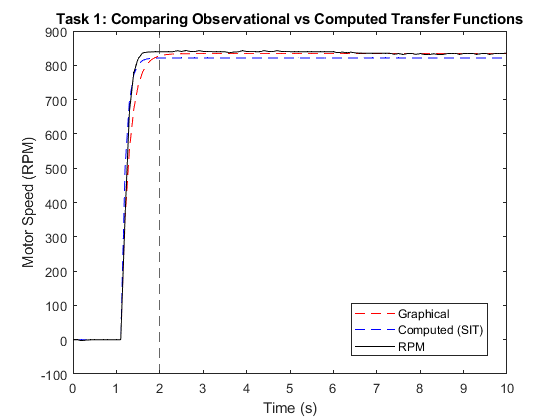
\includegraphics[width=0.6\textwidth]{q1-graphs.png}
    \caption{Step responses of transfer functions }
    \label{fig:q1-graph}
\end{figure}
\par The performance of the both functions were compared by calculating the mean-squared errors (MSEs) $\epsilon$ for each in a given timeframe:
\begin{itemize}
    \item Transient-state error ($0 < t <= 2$): the computed transfer function MSE was found to be $\epsilon_{ts-c} = 3.77 \times 10^4$, while the graphically-found transfer function's MSE was found to be $\epsilon_{ts-g} = 1.66 \times 10^4$. Overall, the MSE was 227\% higher using the SIT-calculated transfer function than the graphically-calculated transfer function.
    \item Steady-state error ($t > 2$): the SIT-calculated transfer function's MSE during the steady-state operation was found to be $\epsilon_{ss-c} = 243.0$ and the graphically-found transfer function's MSE during steady-state operation was $\epsilon_{ss-g} = 17.6$. Overall, there was a 1381\% increase in the MSE value of the SIT-calculated transfer function compared to the graphically-calculated transfer function.
    \item Overall error ($t > 0$): the total MSE for the SIT-calculated transfer function was $\epsilon_{T-c}=3.94\times10^{3}$ while the overall MSE for the graphically-calculated transfer function was $\epsilon_{T-g}=1.66\times10^{3}$. Overall, the total MSE was 237\% larger for the SIT-calculated transfer function than for the graphically-generated function.
\end{itemize}
\par Having evaluated the errors, further tasks were performed using the graphically-generated transfer function, as it outperformed the SIT-generated function for both transient and steady-state parts.
\par Upon observation of the motor function, the motor had a 0.1 second delay, thus the transfer function needed to be multiplied by $e^{-0.1s}$ to account for this delay.
\par The final design allowed for the produced output to be a smooth 1st order response, which enabled further analysis and tuning of the system in the subsequent tasks.
\par The open-loop Simulink model used to obtained the results discussed in this section is shown in \textit{Figure \ref{fig:q1-model}}.\\
\begin{figure}[h!]
    \centering
    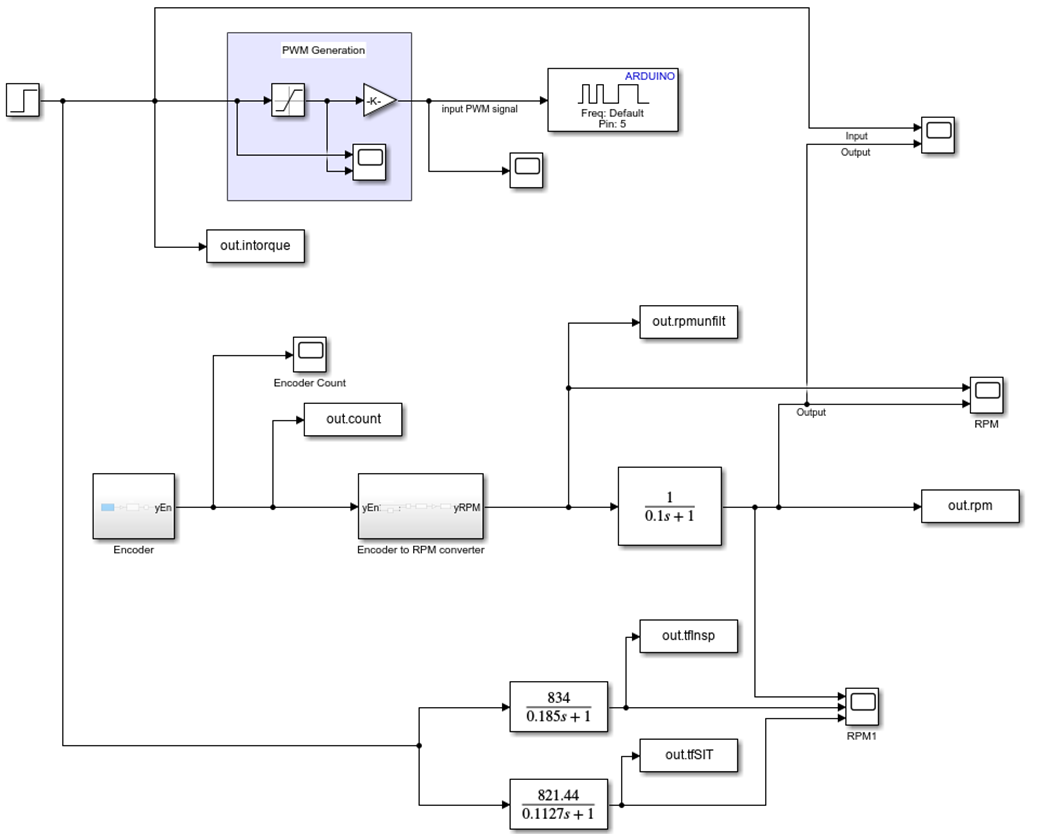
\includegraphics[width=0.75\textwidth]{q1-model.png}
    \caption{The model used to obtain the measures}
    \label{fig:q1-model}
\end{figure}
\section*{Question 2}
\par Using the transfer function obtained in Question 1, closed-loop analysis of the system was used to obtain the required constants for proportional-integral (PI) control. The Ziegler-Nichols method was chosen due to its ease of implementation.
\par An initial PI system was created with $K_p$ and $K_i$ both set to zero. $K_p$ was slowly increased in increments of 0.001, until consistent oscillations were produced in response to a step input. At $K_p = 0.016$, constant oscillations occurred. The system response using the oscillatory $K_p$ is shown in \textit{Figure \ref{fig:q2-oscillatory}}.
\begin{figure}[h!]
    \centering
    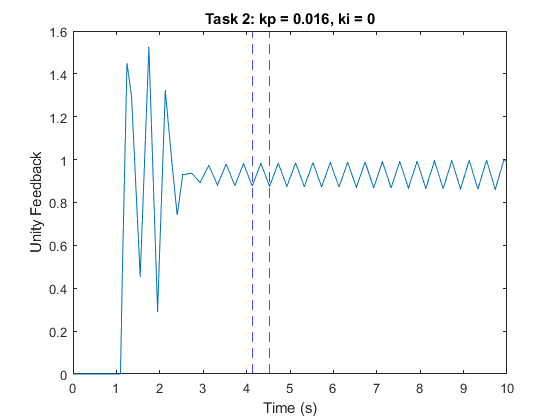
\includegraphics[width=0.6\textwidth]{q2-g1.png}
    \caption{The oscillatory graph used in the Ziegler-Nichols tuning}
    \label{fig:q2-oscillatory}
\end{figure}
\par The peak-to-peak time was measured to obtain the ultimate time period $P_u = 0.407$ s, giving an ultimate gain of $K_u = 0.016$.
\par The Ziegler Nichols tuning equations were applied to obtain the controller values of $K_p$ and $K_i$. The response of the system using the calculated $K_p$ and $K_i$ is shown in \textit{Figure \ref{fig:q2-first}}. An important consideration is that the produced $K_i$ value produced unstable step responses, so it was scaled down by an order of magnitude of two to obtain a stable plot.
\begin{align*}
    K_p & = 0.45 * K_u = 0.45 * 0.016 = 0.0072   \\
    K_i & = 0.83 * P_u = 0.83 * 0.407459 = 0.338
\end{align*}
\begin{figure}[h!]
    \centering
    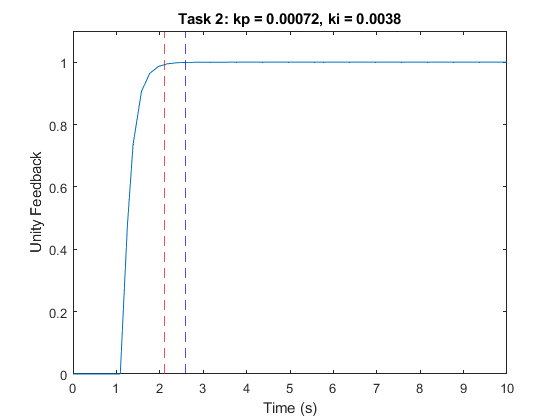
\includegraphics[width=0.6\textwidth]{q2-g2.png}
    \caption{The step response with scaled $K_i$, obtained from Ziegler-Nichols method.}
    \label{fig:q2-first}
\end{figure}
\par The $K_p$ and $K_i$ values were then adjusted by multiplying both by the sample time $T_s = 0.1$s to produce $K_p = 0.00072$ and $K_i = 0.0338$.
\par Upon testing these values, the output displayed violent oscilations. Hence, $K_i$ was once again scaled down by a magnitude of 10. When implemented, this produced the step response depicted in \textit{Figure \ref{fig:q2-second}}.
\par Whilst the settling time was within the required parameters, the peak time exceeded the 1 second requirement, hence $K_i$ was increased to 0.005.
\begin{figure}[h!]
    \centering
    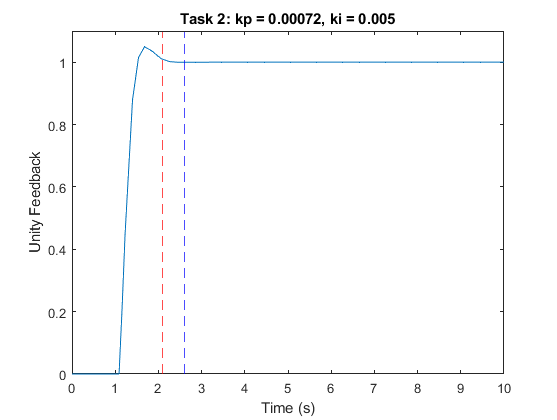
\includegraphics[width=0.6\textwidth]{q2-g3.png}
    \caption{Step response of an adjusted $K_i$ to meet the response requirements.}
    \label{fig:q2-second}
\end{figure}
\par Finally, for open loop analysis, a step input of magnitude 1 was used. However, in a closed-loop system a reference speed was required. Hence, a block of gain $K=834$ (the steady state gain, observed in open loop analysis) was used to scale the output. The step response of the tuned model is shown in \textit{Figure \ref{fig:q2-third}}.
\begin{figure}[h!]
    \centering
    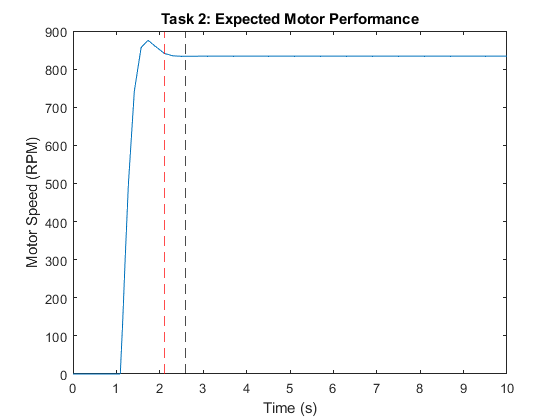
\includegraphics[width=0.6\textwidth]{q2-g4.png}
    \caption{Step response, expected from the motor.}
    \label{fig:q2-third}
\end{figure}
\par The Simulink model that was used to generate the plots is presented in \textit{Figure \ref{fig:q2-model}}.
\begin{figure}[h!]
    \centering
    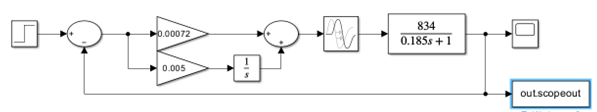
\includegraphics[width=0.75\textwidth]{q2-model.png}
    \caption{The model used to obtain the plots.}
    \label{fig:q2-model}
\end{figure}
\section*{Question 3}
\par After having the simulated model working, the next step was to integrate it on the Arduino to check against the posed requirements and physical constraints.
\begin{figure}[h!]
    \centering
    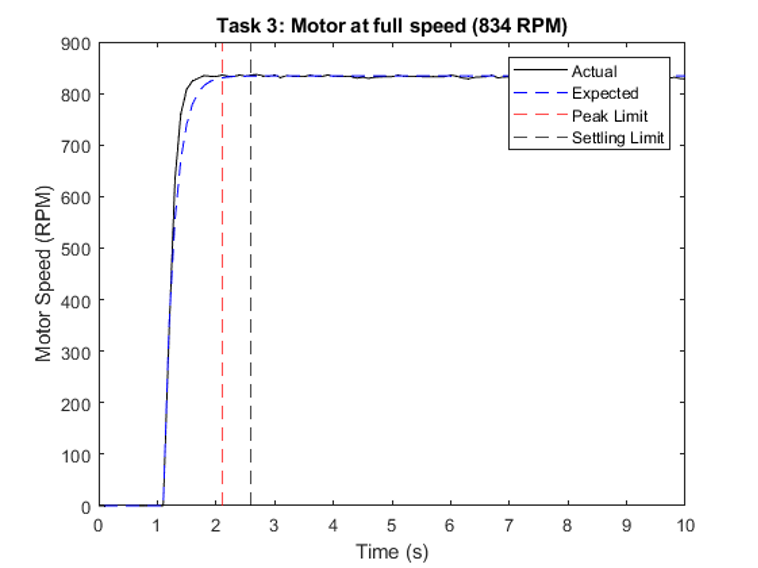
\includegraphics[width=0.6\textwidth]{q3-g1.png}
    \caption{The step response of the motor at full speed with a PI controller.}
    \label{fig:q3-first}
\end{figure}
\par As observed \textit{Figure \ref{fig:q3-first}}, the response in simulation was very close to the actual response generated by the motor. The response stabilised well within the peak limit and settling limit and showed no overshoot of the steady-state value. In fact, it reached the steady-state faster than the simulated response, with a settling time of around 0.8 seconds, compared to 1.28 seconds for the simulated response. This confirmed that the chosen values for the PI controller were accurate and produced the desired results. In order to further verify the accuracy of the controller, different motor speeds were tested. These produced more varied results as shown in \textit{Figures \ref{fig:q3-second} and \ref{fig:q3-third}}.
\begin{figure}[h!]
    \centering
    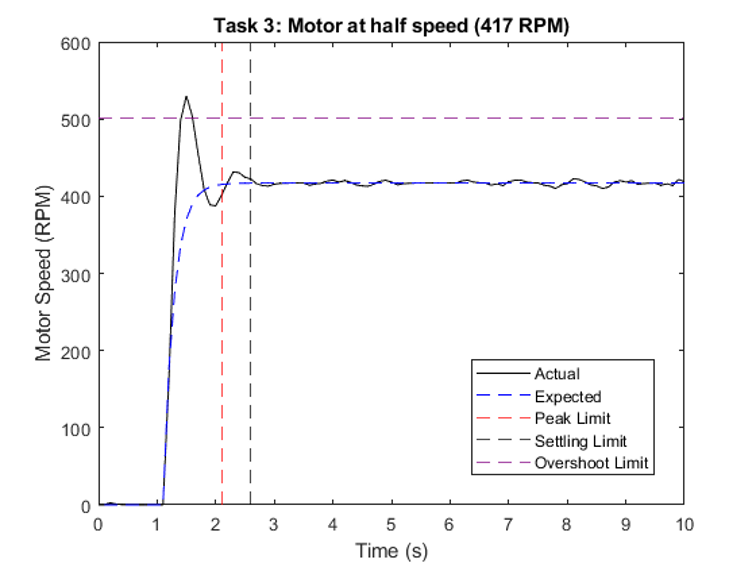
\includegraphics[width=0.6\textwidth]{q3-g2.png}
    \caption{The motor's response to a half step input.}
    \label{fig:q3-second}
\end{figure}
\par Comparing the performance of the motor to the simulated response with PI control applied, there appeared to be significant overshoot when run at half speed which was not present in the full speed response. As shown in \textit{Figure \ref{fig:q3-second}}, a peak value of 524 RPM was reached, which exceeded the overshoot limit of 20\%, and only just stabilised within the settling time limit. This proved that at lower speeds, the PI controller did not perform as robustly in real-life as it did in simulation, and showed that there was still room for improvement of the controller. To confirm these findings, the motor was also tested at a quarter speed. The results of this experiment are below.
\begin{figure}[h!]
    \centering
    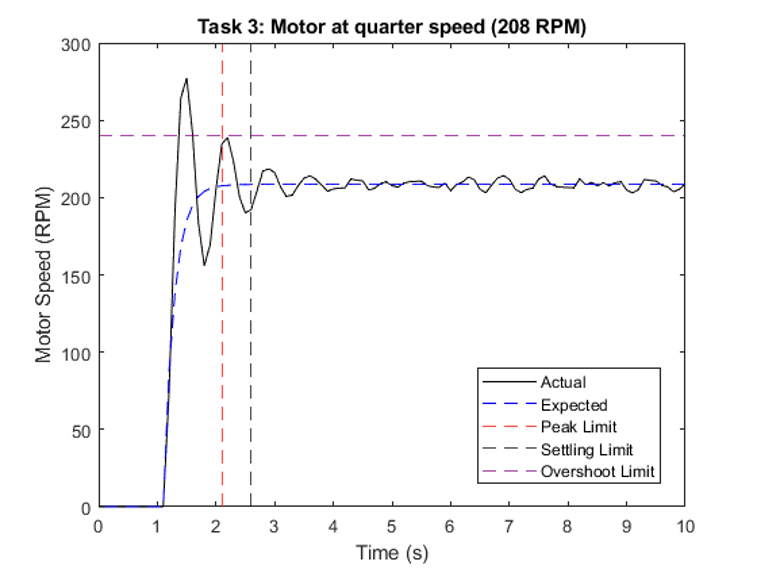
\includegraphics[width=0.6\textwidth]{q3-g3.png}
    \caption{The motor's response to a full step input.}
    \label{fig:q3-third}
\end{figure}
\par The results in \textit{Figure \ref{fig:q3-third}} show that the PI controller did not meet any of the specifications when the motor was run at a quarter speed. The overshoot of 275 RPM was far too high, and showed much more oscillation before a steady-state was eventually reached. This was far from the predicted response gained using the transfer function, and prompted exploration into why these discrepancies might have occurred.
\par The primary reason for a difference between the performance of the motor in simulation and in the real-world is due to the fact that the mechanical properties of the device are difficult to model in simulation. Electrical properties can be modelled with greater accuracy, but parameters such as friction which could act against the rotor torque, thereby reducing the motor speed and limiting the current through the coils, is much more difficult to predict. Typically, friction effects are less noticeable at higher speeds, and have a much greater impact at lower speeds. Coulomb friction and viscous friction are two such examples. Coulomb friction opposes motion and is always present, and is independent of velocity. Viscous friction is dependent on velocity, and therefore increases as velocity increases \cite{Virgala2013}.
\par Additionally, non-linearities inherent in the behaviour of the motor are assumed to be negligible when designing the model and generating a linear transfer function. This is because it is more convenient and is often sufficient for conventional control problems. However, this non-linear behaviour in certain regions of operation, make the PI controller difficult to tune for real-world usage, as the effects of friction are highly varied and dependent on parameters which are not easily modelled. Once such example of this is demonstrated well by the graphs at lower motor speeds, where static friction is particularly challenging to overcome. Static friction is an effect which occurs when a component has been inactive for a certain period of time, and therefore requires a greater force to start the relative motion than the force which is required to sustain this motion. This effect is demonstrated well by the longer settling time shown at lower motor speeds than that of the motor running at full speed, proving that more force was required to start the motor and overcome the static friction \cite{ijsrpStudyNonlinear}.
\section*{Question 4}
\par To compensate for some of the controller weaknesses encountered in previous chapter, a variety of techniques were explored – some of which are discussed below. The techniques were used individually and not coupled to explore their effect on the PI controller.
\subsection*{PID Control}
\par The PI controller performed optimally at full speed, however it showed more variation when the motor was run at half speed and quarter speed with regard to overshoot and oscillations in the transient response. This showed that further tuning was necessary, thus PID control was explored as a method to overcome these shortcomings. The intention of adding the derivative controller was to reduce overshoot, as derivative gain is proportional to the rate of change of the process variable, so acts to reduce output when the process variable is increasing quickly. The tuning of this gain parameter followed an offline trial and error approach, as values could be tested more quickly and safely than the online equivalent. Once a suitable order of magnitude was determined in simulation, more specific values were tested using the motor. The ideal order of magnitude for the derivative gain was found to be $10^{-5}$, thus the gain was slowly increased from $0.00001$ in increments of $0.000005$, with the motor running at half speed until the optimal response was reached. The $K_i$ and $K_p$ values were left unchanged, and this resulted in a $K_d$ value of 0.00004 producing the best response at lower motor speeds.
\begin{figure}[h!]
    \centering
    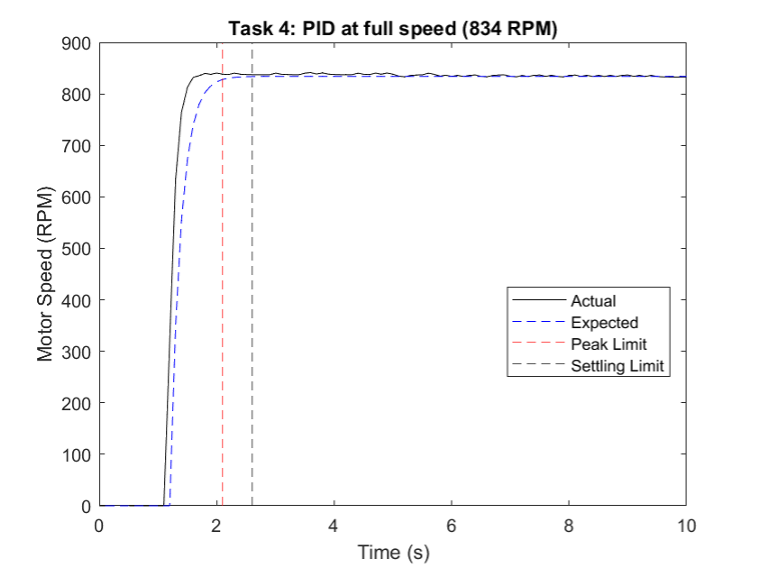
\includegraphics[width=0.6\textwidth]{q4-pid1.png}
    \caption{The motor's response at full-speed, using PID.}
    \label{fig:q4-pid1}
\end{figure}
\par With PID control applied, the step response in \textit{Figure \ref{fig:q4-pid1}}. As shown by the graph, there is no overshoot of the steady state value, and the settling time of 884 ms falls adequately within the settling time limit. This is very similar to the response seen using PI control, and confirms that the PI values chosen for this controller were correct.
\begin{figure}[h!]
    \centering
    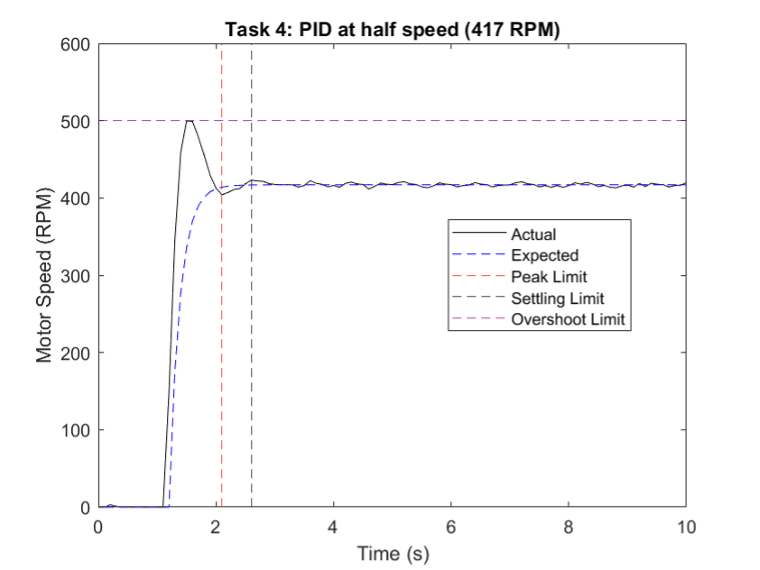
\includegraphics[width=0.6\textwidth]{q4-pid2.png}
    \caption{The motor's response at half-speed, using PID.}
    \label{fig:q4-pid2}
\end{figure}
\par The graph in \textit{Figure \ref{fig:q4-pid2}} shows vast improvement in the desired areas, with a settling time and overshoot within the predetermined limits. The response shows an overshoot of just under 20\%, as it reaches 499 RPM, and just settles within the required $1.5 \text{s}$. Although this controller only just fulfils the requirements, any corrections to individual aspects appeared to come at the expense of deteriorating other areas of the response. For example, although increasing the derivative gain effectively reduced overshoot, it resulted in greater oscillations in the steady state part of the response, and a slightly longer settling time. For this reason, the values of $K_p$, $K_i$ and $K_d$ were chosen such that the controller remained just within the overshoot and settling time limits, whilst maintaining a smoother steady state response at the desired RPM.
\begin{figure}[h!]
    \centering
    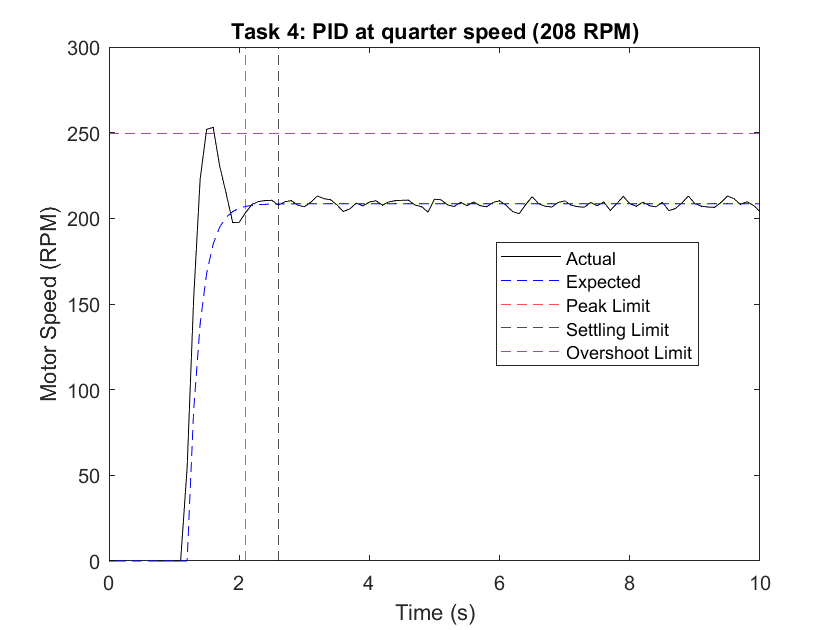
\includegraphics[width=0.6\textwidth]{q4-pid3.png}
    \caption{The motor's response at quarter-speed, using PID.}
    \label{fig:q4-pid3}
\end{figure}
\par In \textit{Figure \ref{fig:q4-pid3}}, the step response using PID control again showed improvement to the PI control output, which displayed greater overshoot and oscillated much more in the transient part of the response than the result using PID control. A peak speed of 261 RPM was reached, which was just beyond the desired 20\% overshoot limit, and the same was true of the settling time, which appeared to occur at around 1.5 s. Similarly to the results at half speed, a compromise between the optimisation of these factors was reached, with the Kp, Ki and Kd values chosen such that overshoot was limited while keeping oscillations in the steady state to a minimum, and remaining just within the settling time bounds.
\subsection*{Model Predictive Control Integration}
\par To further improve upon the controller design for our group task, we decided to utilise the Model Predictive Control (MPC) method in Simulink, this was obtained by installed the Model Predictive Control Toolbox in MATLAB.
\par Model Predictive Control systems operates by using numerically minimising a cost function of a plant provided to it, to generate output predictions over a finite time horizon, continuously iterating over time \cite{Nikolaou2001}.
\par A typical MPC system contains an input-output system to control, in this instance it’s the DC powered motor where the input is voltage \& output is torque.
\begin{figure}[h!]
    \centering
    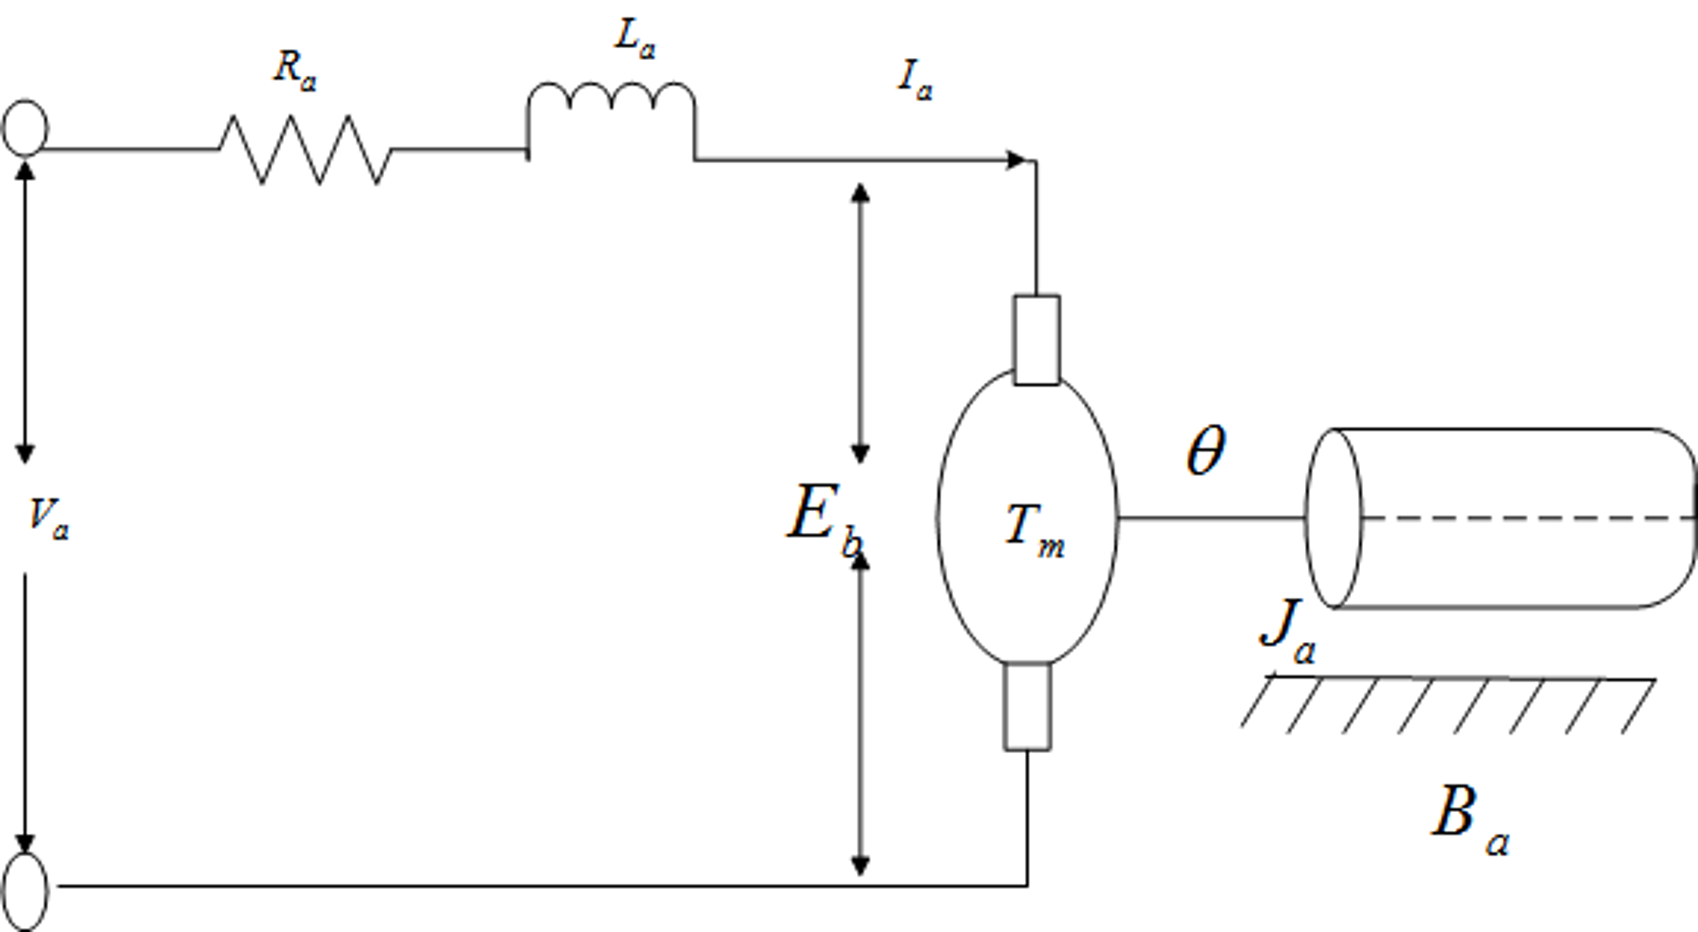
\includegraphics[width=0.6\textwidth]{q4-schematic.png}
    \caption{DC motor circuit schematic \cite{article}}
    \label{fig:q4-schematic}
\end{figure}
\par MPC is an improvement as it computes predicted future output values and computes a predicted future error as input for its cost-function optimizer. The optimizer will produce new inputs for the model and feed the model the input value that produces the least error. The cost-function optimizer does this by enforcing the constraints of the system (the first order equations derived from the transfer function that represents the DC motor system offline) \cite{libretexts123MIMO}.
\par This reduces overall control effort of the system, in comparison to traditional PI/PID controllers and thus better overall responses, regarding peak time, settling time \& percentage overshoot. The parameters used in the MPC and the response parameters are summarised in \textit{Tables 1} and \textit{2}.
\begin{table}[h!]
    \centering
    \begin{tabular}{| c | c | c | c |}
        \hline
        \textbf{Ts} & \textbf{PredictionHorizon} & \textbf{ControlHorizon} & \textbf{Weights.ManipulatedVariables } \\
        \hline
        0.1         & 2                          & 1                       & 0.5                                    \\
        \hline
    \end{tabular}
    \caption{The parameters used for MPC set-up.}
    \label{table:simulation-inputs}
\end{table}

\begin{table}[h!]
    \resizebox{\textwidth}{!}{
        \begin{tabular}{| c | c | c | c | c | c |}
            \hline
            \textbf{Mode} & \textbf{Settle Value, rpm} & \textbf{Peak Value, rpm} & \textbf{Overshoot, \%} & \textbf{Peak Time, s} & \textbf{Settling Time, s} \\
            \hline
            Full-Speed    & 834                        & 839                      & 0.6                    & 0.7                   & 0.7                       \\
            \hline
            Half-Speed    & 538                        & 597                      & 11.0                   & 0.4                   & 1.2                       \\
            \hline
            Quarter-Speed & 265                        & 351                      & 32.5                   & 0.3                   & 1.8                       \\
            \hline
            Tenth-Speed   & 48                         & 64                       & 33                     & 1.4                   & 2.9                       \\
            \hline
        \end{tabular}}
    \caption{The parameters used for MPC set-up.}
    \label{table:simulation-inputs}
\end{table}
\begin{figure}[h!]
    \centering
    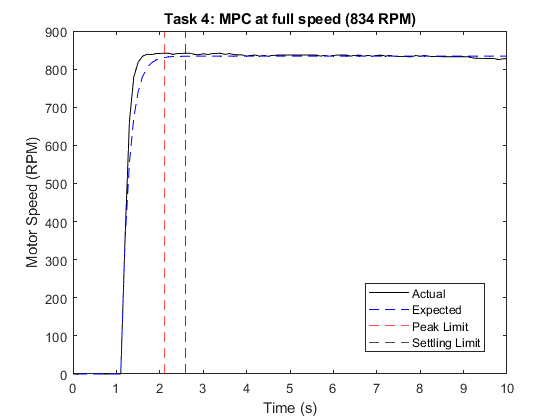
\includegraphics[width=0.48\textwidth]{q4-g1.png} 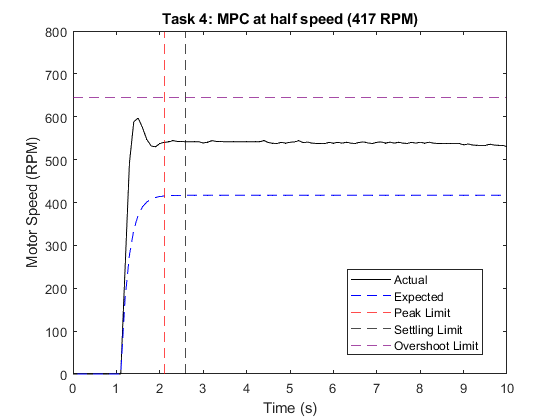
\includegraphics[width=0.48\textwidth]{q4-g2.png}
    \caption{The motor's response at full-speed, using PID.}
    \label{fig:q4-g1}
\end{figure}
\begin{figure}[h!]
    \centering
    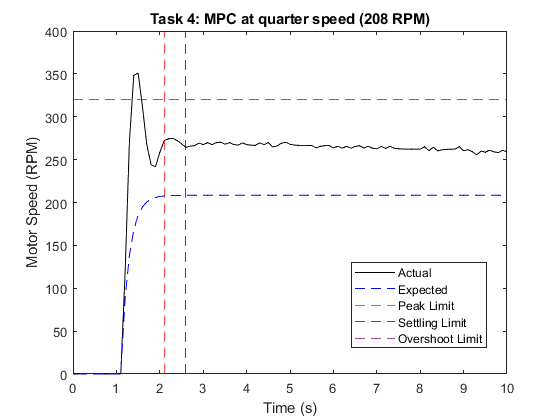
\includegraphics[width=0.48\textwidth]{q4-g3.png} 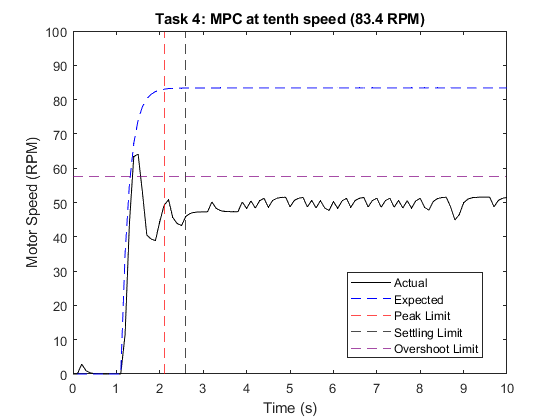
\includegraphics[width=0.48\textwidth]{q4-g4.png}
    \caption{quarter and tenth speeds}
    \label{fig:q4-g2}
\end{figure}
\subsection*{Phase Lead Compensators}
\par To compensate for the overshoot present in the response while using the PI controller, our team decided to develop a phase lead compensator (PLC). PLCs are used to improve the stability of feedback control systems and aims to increase the response speed \cite{sciencedirectLeadCompensator}. Which in context for this project equates to the settling time. This was the primary justification to pursue this design.
\par Lead compensators are designed to be implemented into a system in transfer function form, so the derivation comes from a root-locus of a typical PLC \cite{umichControlTutorials1}:
\begin{align*}
    C(s)=\frac{K_c(s-z_0)}{(s-p_0)}
\end{align*}
\par For consistency an identical plant function  of $(\frac{834}{0.185s\ +\ 1})$ was used for implementation. A first order lead compensator contributes one pole and one zero to the loop, in the case of a lead compensator $z_0<p_0$. An iterative process was then used to tune the controller. There are three tuneable parameters for this model. $K_C$, $z$ and $p$. Upon inspection, $K_C$ set the steady state value of the system. Varying $p$ would alter the steady state and varying $z$ would alter the settling time, at the expense of a small overshoot ($\ll20$\%). Initially the best trials came from when $p_0=0$. This was the best $p$ value to consistently maintain the ideal steady state value. Therefore, the transfer function simplified as follows:
\begin{align*}
    C\left(s\right)=\frac{K_c\left(s-z_0\right)}{(s-p_0)}=\frac{K_cs-K_cz_0}{s}=\frac{K_cs}{s}-\frac{K_cz_0}{s}=\ K_c-\frac{K_cz_0}{s}
\end{align*}
\par Upon consideration the transfer function of this controller appears to behave like a basic PI controller and thus no significant improvements could be made with these parameters.
\begin{align*}
    PI=K_p+\frac{K_i}{s}\ \ \approx\ K_c-\frac{K_cz_0}{s}
\end{align*}
\par Therefore the parameters had to be further iterated with $p$ not equal to zero, and it was found that values of $K_C = 0.0012$, $p= 0.01$, $z= -5.5$ improved the settling time at full speed (834 RPM) and was successfully implemented on the motor (\textit{Figure \ref{fig:q4-phase}}). However, upon analysis the results got significantly worse at lower motor speeds, rendering the controller design unusable at these speeds due to high oscillatory behaviour. Therefore, further research and improvements are needed before this model type could outperform other methods presented in this report.
\begin{figure}[h!]
    \centering
    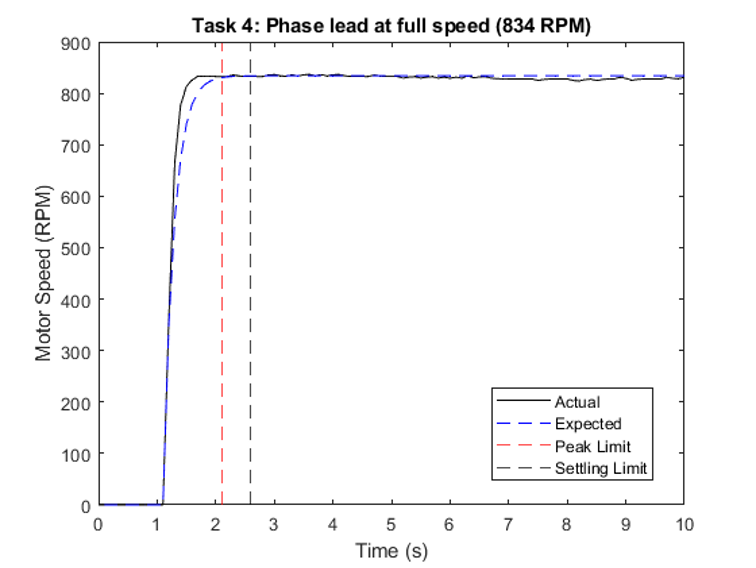
\includegraphics[width=0.6\textwidth]{q4-phase.png}
    \caption{DC motor circuit schematic \cite{article}}
    \label{fig:q4-phase}
\end{figure}
\newpage
\bibliographystyle{IEEEtran}
\bibliography{References}
\end{document}